%% eval.tex
%% $Id: eval.tex 61 2012-05-03 13:58:03Z bless $

\chapter{Evaluation}
\label{ch:Evaluation}
%% ==============================
In this evaluation section, we explore how well the algorithm performs by looking at the performance and examining the decompositions.
Our primary interest lies in two aspects, the size of the factors contributing to the decomposition and the coverage of final states by each factor.
Through this analysis, we aim to gauge the algorithm's effectiveness in generating meaningful decompositions.
This evaluation is pivotal for understanding the algorithm's capability to produce concise and relevant factors, providing insights into the temporal structure of the given labels.
For this purpose, the complete f2f dataset was evaluated, described in Section \ref{ch:prelimiaries:real-world-data} consisting of 62 Temporal graphs with 20 to 56 edges each, ignoring loop edges.
In total, there are 3321 edges with a combined label length of around 2.3 million giving an average label length of 6993.
Please note that the data sets represent people looking at each other, a directed edge from node $u$ to $v$ indicates participant $u$ looks at participant $v$ therefore only one edge label at a given time step $t$ has its value set, $\tau(e)[t] = 1$ for exactly one outgoing edged of $u$.
This is also visible in the data as only 13.4\% of values in the labels is set to 1 over all the labels.

\section{Performance Evaluation}
\label{ch:Evaluation:performance}
Although performance was not the main focus of the implementation and evaluation, generating \orDecomp for the complete dataset is reasonably fast with around 3 seconds if using the maximal divisors or the greedy approach.
The Fourier-transformation takes a lot of additional time for cleaning multiples of a factor as well as replacing factors with multiple set values with a set of factors with only one set value, causing it to run for 1 minute and 45 seconds.
All benchmarks were performed on an AMD Ryzen 5 2600X six-core processor (12 threads) with a 3.6 GHz base clock and a 4.2 GHz boost clock speed. For memory, 16GB 3200MHz RAM and a Samsung EVO SSD was used for persistent storage.
\begin{table}[h]
	\begin{tabular}{l|rrr}
		 & MaxDivisors & GreedyShortFactors & FourierTransform  \\
		\hline
		 OR-Decomposition & 3.12 & 3.47 & 105 \\
		 AND-Decomposition & 9.85 & 24.83 & - \\
		 	
	\end{tabular}
	\caption{Decomposition time in seconds [s] for complete dataset}
	\label{tab:eval-performance}
\end{table}
It is to be noted that the \andDecomp is expected to be slower because of the considerably greater amount of zeros in the data set as well as the modification to the cover finding algorithm.
While with an \orDecomp, each additional factor can only remove outliers, in an \andDecomp an additional factor can also add new outliers.
Because of that, the current outliers of a decomposition must be recalculated considering all factors.
The Fourier-transform method again increases the number of factors per cover, which hurts performance.
Also, it is not implemented for \andDecomp as it is not considered reasonable, since a human would still need to look at all factors since it is an \andDecomp.

\section{Decomposition Evaluation}
\label{ch:Evaluation:decomposition-quality}
Moving on to the decomposition evaluation, we validate each method separately and then compare them against each other.
We also benchmark \andDecomp and \orDecomp.
To get an insight into how well a particular decomposition method is performing, decompose the whole data-set and then plot each factor of each decomposition by its relative size compared to the original \DFA size and the relative amount of covered values of the \DFA by this factor.
\begin{figure}[t]
	\begin{minipage}[h]{0.49\linewidth}
		\centering
		OR-decomposition
		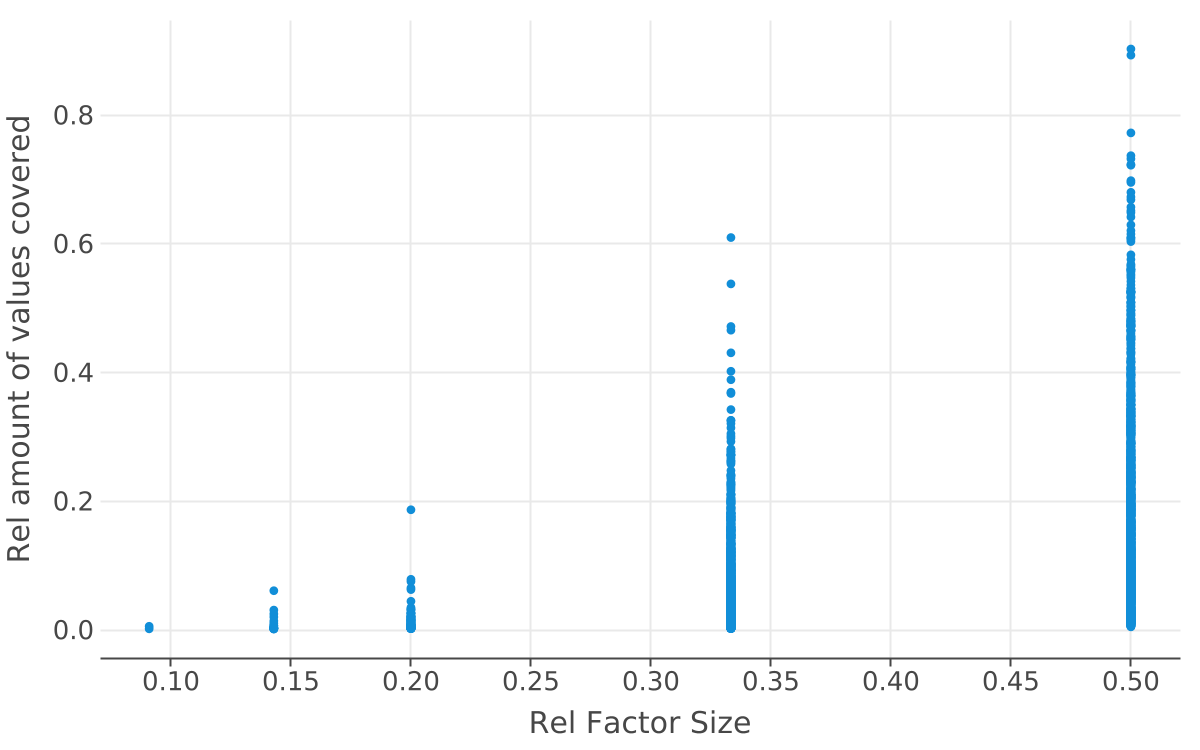
\includegraphics[width=\linewidth]{../plots/point-plots/MAX_DIVISORS-OR-all-relative-values-by-factor-size.png}
	\end{minipage}
	\begin{minipage}[h]{0.49\linewidth}
		\centering
		AND-decomposition
		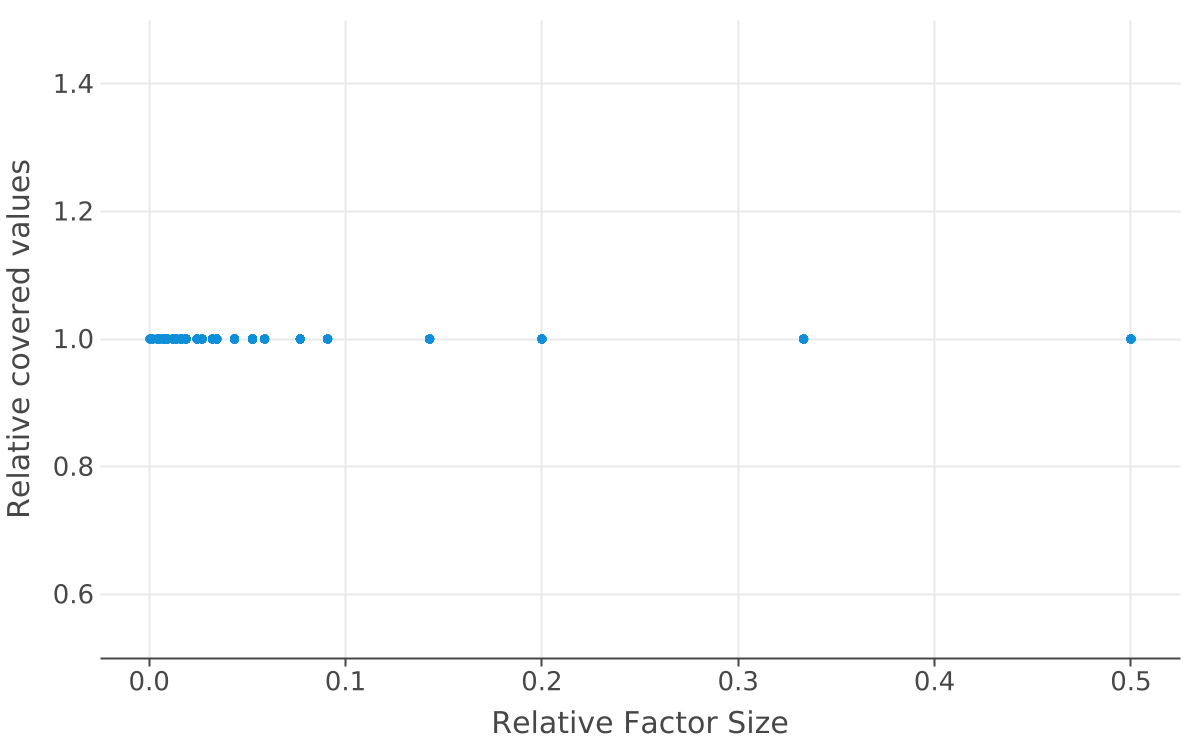
\includegraphics[width=\linewidth]{../plots/point-plots/MAX_DIVISORS-AND-all-relative-values-by-factor-size.png}
	\end{minipage}
	\caption{Relative amount of covered values by relative factor size}
	\label{fig:eval:max-divisor-all-factors}
\end{figure}

\subsection{Maximal Divisor Decomposition Evaluation}
\label{ch:Evaluation:decomposition-quality:max-divisor}
Decomposing with the Maximal Divisor method implemented as described in Section \ref{ch:Implementation:max-divisor} was used first for decomposing the complete dataset.
Analyzing the resulting decompositions and plotting each factor $B_i$ of each decomposition of a \DFA $A$ by its size relative to the original $\frac{|B_i|}{|A|}$ with its relative amount of covered final states from $A$, the precision up to that factor.
The results are shown in Figure \ref{fig:eval:max-divisor-all-factors} and it clearly shows that the \orDecomp finds factors, but there are fewer factors in the decompositions and they cover fewer values than the comparable \andDecomp.
\begin{figure}[h]
	\begin{minipage}[h]{0.49\linewidth}
		\centering
		OR-decomposition
		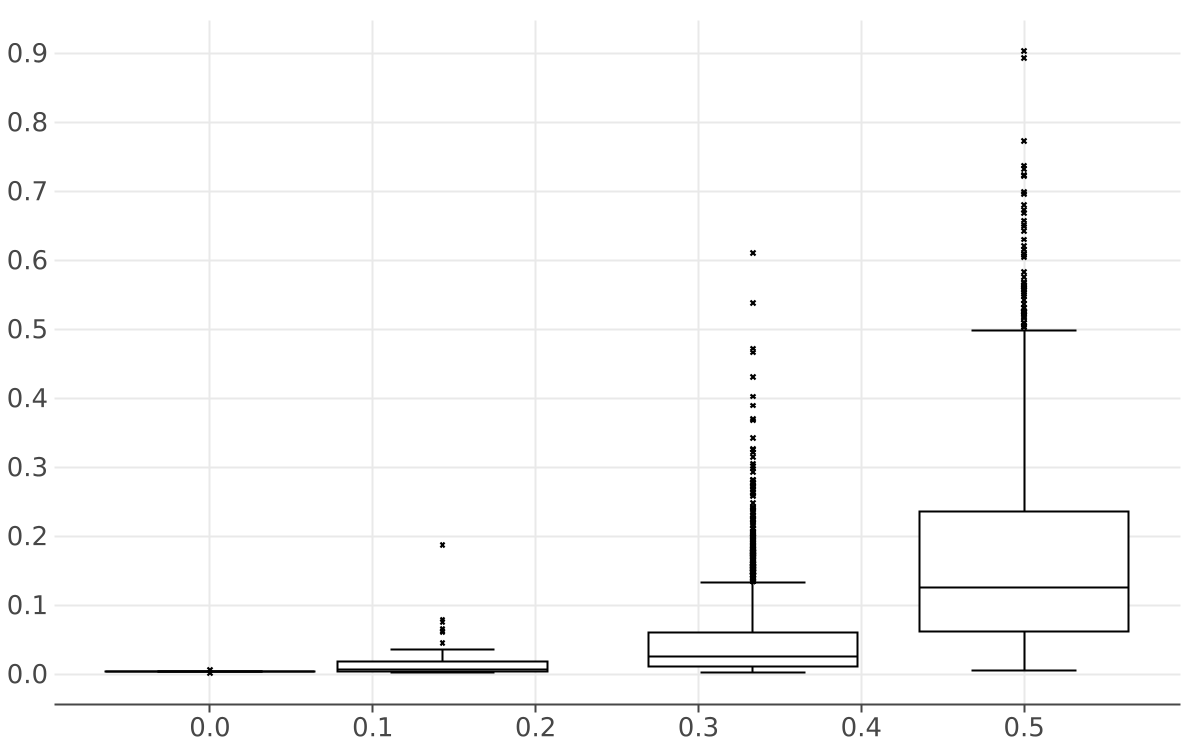
\includegraphics[width=\linewidth]{../plots/box-plots/MAX_DIVISORS-OR-all-relative-values-by-factor-boxplot-dist.png}
	\end{minipage}
	\begin{minipage}[h]{0.49\linewidth}
		\centering
		AND-decomposition
		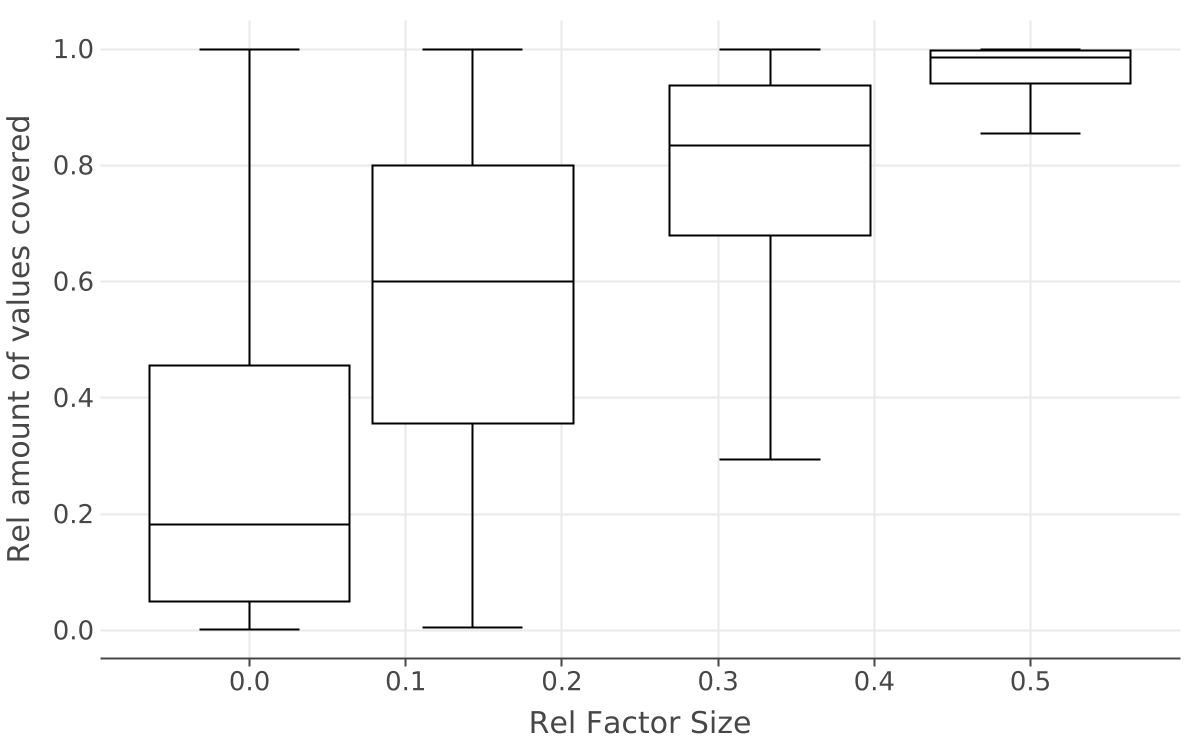
\includegraphics[width=\linewidth]{../plots/box-plots/MAX_DIVISORS-AND-all-relative-values-by-factor-boxplot-dist.png}
	\end{minipage}
	\caption{Relative amount of covered values by relative factor size (MaxDivisors)}
	\label{fig:eval:max-divisor-all-factors-box-plot}
\end{figure}
A lot of data-points collapse onto a single $x$ value since they are grouped by their relative size, not their absolute.
For the \andDecomp there are many values scattered around a small relative factor size.
To get some more insight into the distribution, a box plot is also provided in Figure \ref{fig:eval:max-divisor-all-factors-box-plot}.
Here, the same $x$ and $y$ values are chosen but the values are aggregated such that if a $x$ value is too close to another, their data points get merged.
The \orDecomp shows that even with a relative factor size of $\frac{1}{2}$ which is the largest possible factor, the median over all these factors only covers 10\% of the target \DFA.
There are some outliers with $\frac{1}{3}$ or $\frac{1}{2}$ the original size which covers already up to 60-80\% of the original \DFA but they are outliers and most of the \orDecomp found by using the maximal divisors cover almost nothing of the original, especially the short factors.
For the \andDecomp a lot of the small relative factor sizes have to be aggregated to visualize them as box-plots, so if a relative factor size value is less than $\frac{1}{20}$ away from a previous data-point, they become one distribution.
Notably, factors of size between $\frac{1}{12}$ and $\frac{1}{5}$ stretch over the entire range of relative covered values in the decomposition. With $\frac{1}{6}$ relative factor size, the \andDecomp already covered more than 50\% of a given \DFAs final states.


\subsection{Greedy Short Factor Decomposition Evaluation}
\label{ch:Evaluation:decomposition-quality:greedy-short-factors}
Looking at the novel greedy approach for finding short factors, a similar picture becomes evident.
We find more factors and some better ones as before when using just the maximal divisors as potential factor sizes, but some factor size data points from Figure \ref{fig:eval:greedy-short-factors-all-factors} only have a single factor with that relative size.
Although there are now more factors present overall, the short factors found, only cover at most 20\% of the final states of the \DFA they compose.
\begin{figure}[h]
	\begin{minipage}[h]{0.49\linewidth}
		\centering
		OR-decomposition
		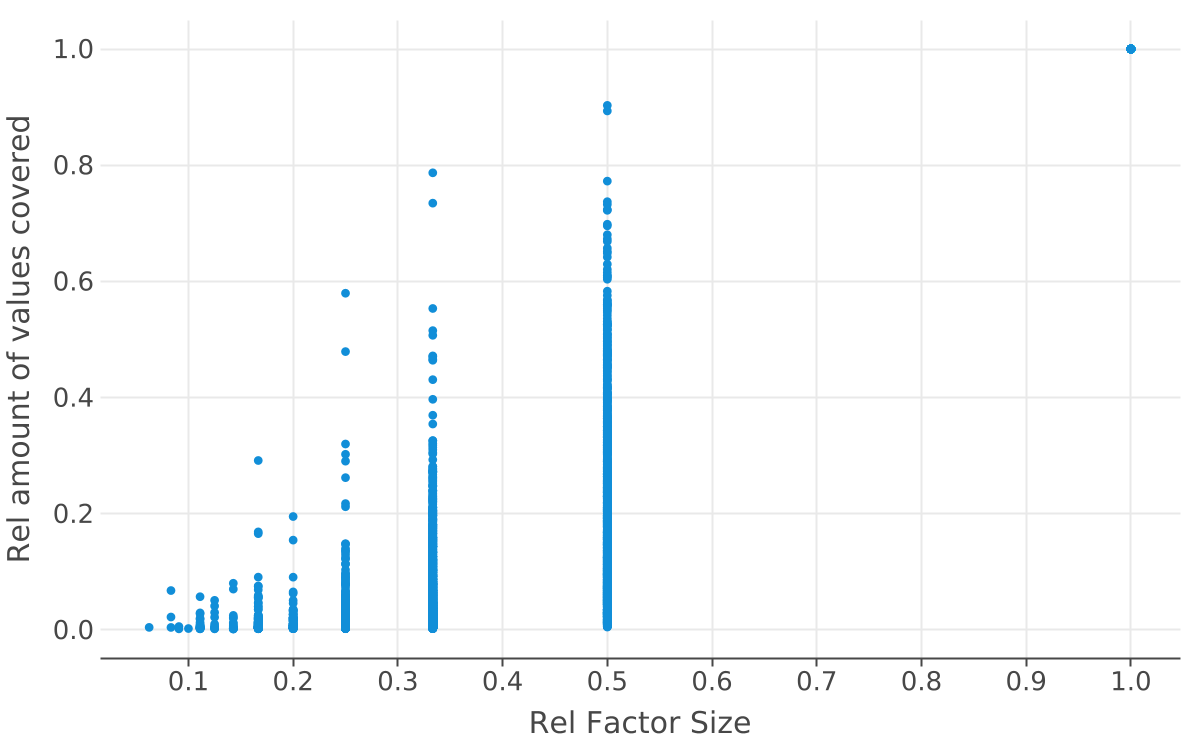
\includegraphics[width=\linewidth]{../plots/point-plots/GREEDY_SHORT_FACTORS-OR-all-relative-values-by-factor-size.png}
	\end{minipage}
	\begin{minipage}[h]{0.49\linewidth}
		\centering
		AND-decomposition
		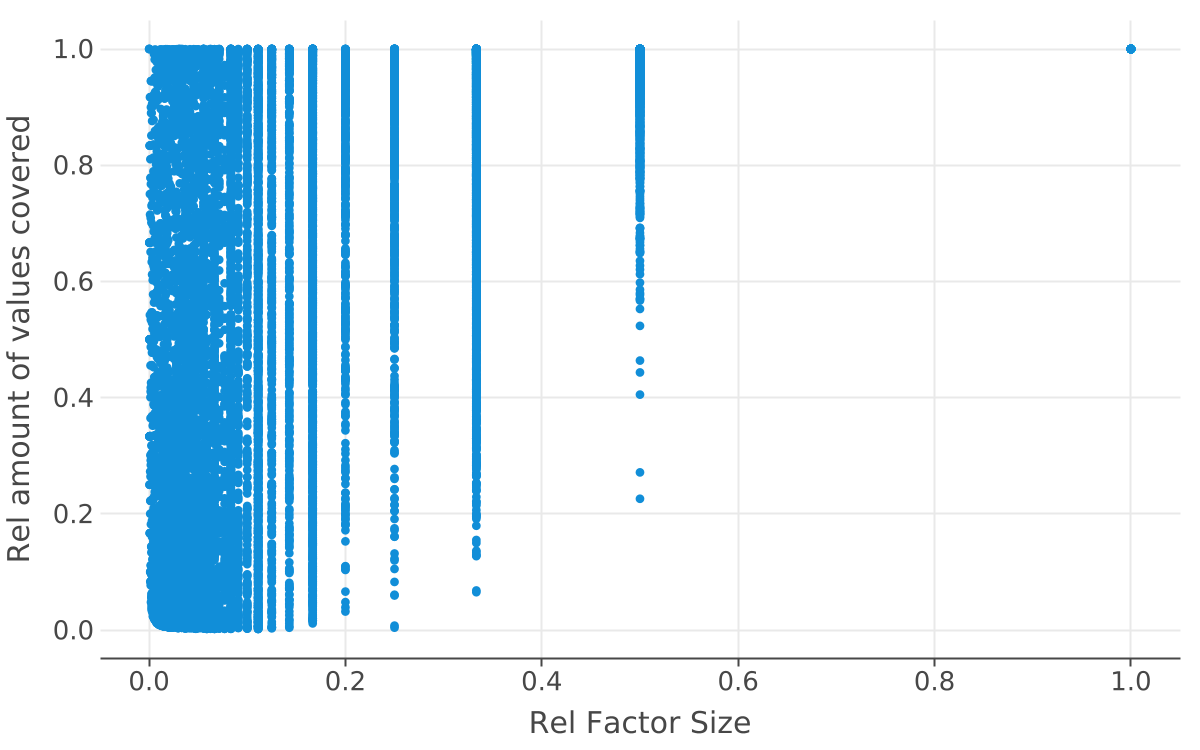
\includegraphics[width=\linewidth]{../plots/point-plots/GREEDY_SHORT_FACTORS-AND-all-relative-values-by-factor-size.png}
	\end{minipage}
	\caption{Relative amount of covered values by relative factor size}
	\label{fig:eval:greedy-short-factors-all-factors}
\end{figure}
As Figure \ref{fig:eval:greedy-short-factors-all-factors-box-plot} shows, we find more factors and even some better outliers of the distribution, but the overall covered values stay very low.
There are factors of relative size $\frac{1}{3}$ or $\frac{1}{2}$ which cover up to 80\% of the final states of their \DFA present, but the median over the distributions never exceed 16\%.
This is partially expected, due to the real world scenario and the way the data is generated.
There are not that many 1 values in the labels, so the probability of them reoccurring after a periodic time is also low.
It is also just not likely that a person looks at another person in a exactly periodic way, the data is temporal but just not very periodic.
\begin{figure}[t]
	\begin{minipage}[h]{0.49\linewidth}
		\centering
		OR-decomposition
		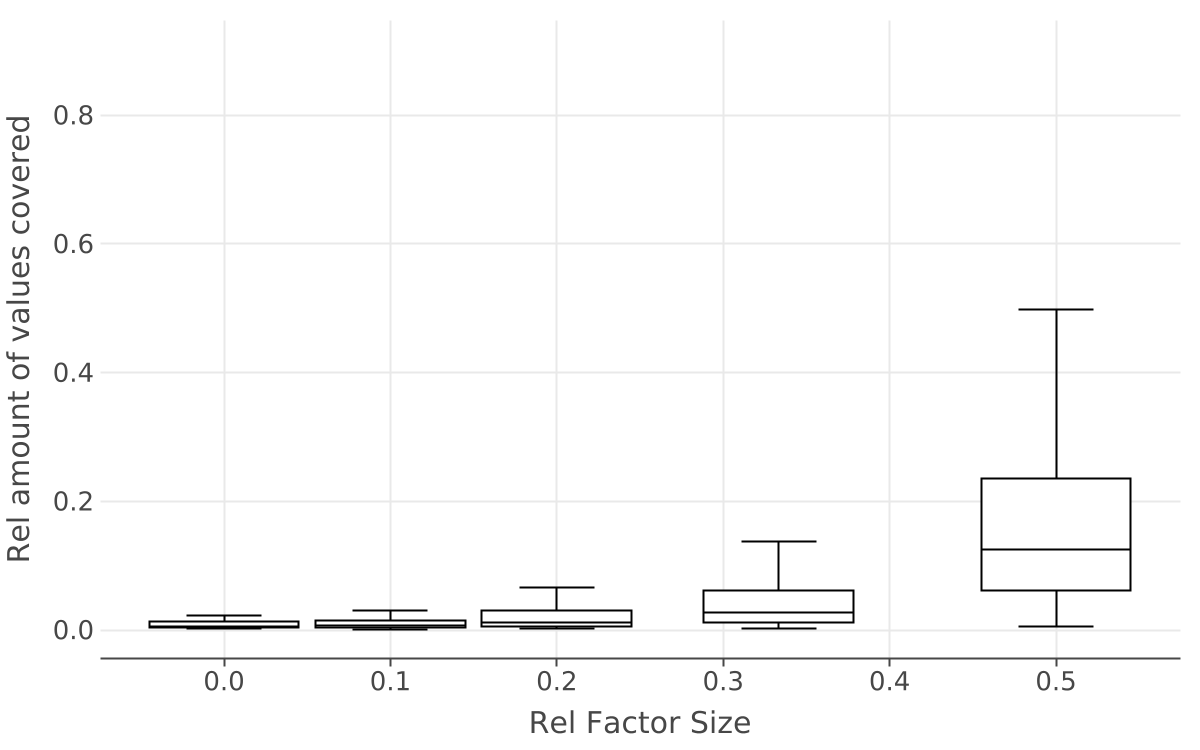
\includegraphics[width=\linewidth]{../plots/box-plots/GREEDY_SHORT_FACTORS-OR-all-relative-values-by-factor-boxplot-dist.png}
	\end{minipage}
	\begin{minipage}[h]{0.49\linewidth}
		\centering
		AND-decomposition
		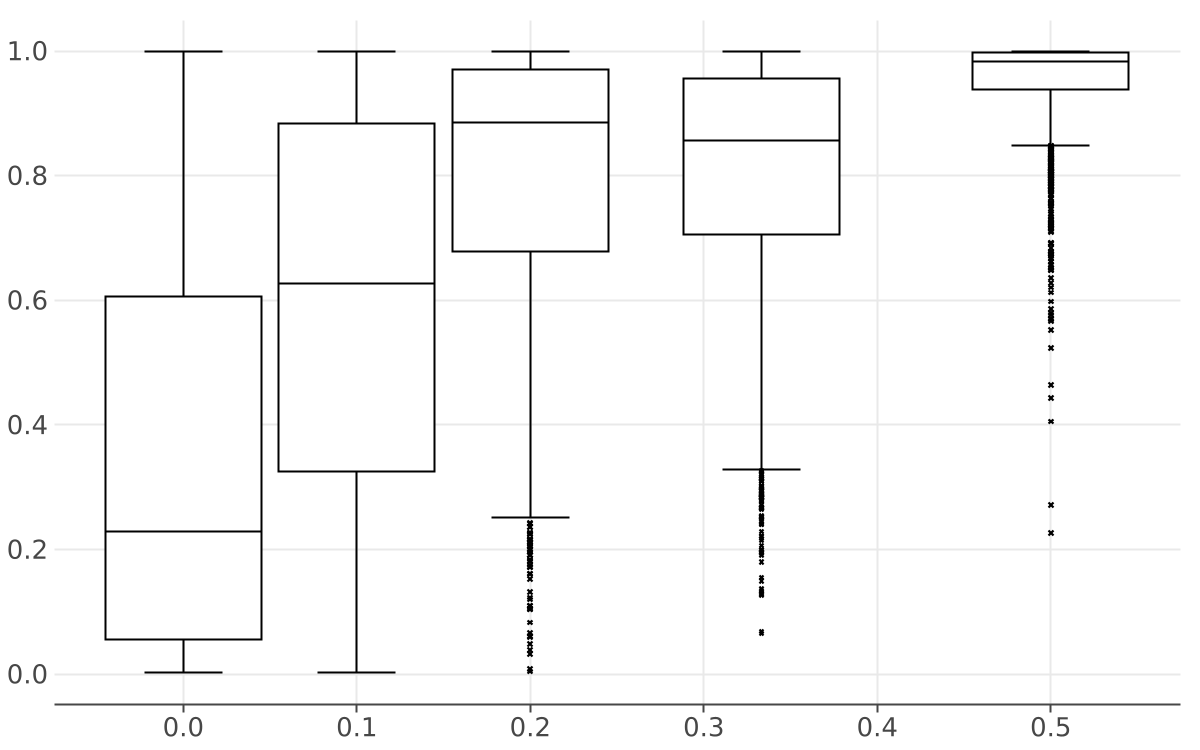
\includegraphics[width=\linewidth]{../plots/box-plots/GREEDY_SHORT_FACTORS-AND-all-relative-values-by-factor-boxplot-dist.png}
	\end{minipage}
	\caption{Relative amount of covered values by relative factor size (GreedyShorFactors)}
	\label{fig:eval:greedy-short-factors-all-factors-box-plot}
\end{figure}


\subsection{Fourier-Transform Decomposition Evaluation}
\label{ch:Evaluation:decomposition-quality:fourier}

\begin{figure}[h]
	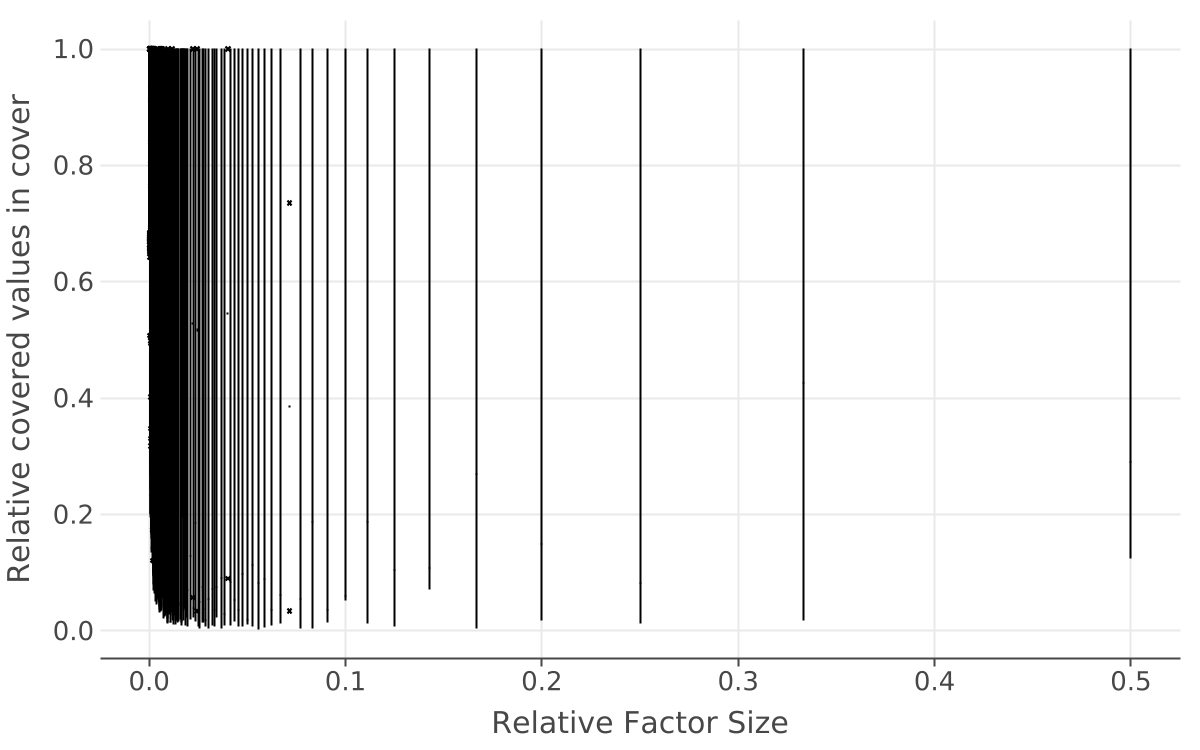
\includegraphics[width=\linewidth]{../plots/box-plots/FOURIER_TRANSFORM-OR-all-relative-values-by-factor-boxplot-outliers.png}
	\caption{Relative amount of covered values by relative factor size (FourierTransform)}
	\label{fig:eval:fourier-all-factors-box-plot}
\end{figure}


\section{Explainability Evaluation}
\label{ch:Evaluation:explainability}

\begin{table}[h]
	\centering
	\begin{tabular}{ll|rr|rrr}
		& &  \multicolumn{2}{c}{DS} & \multicolumn{3}{c}{size}  \\
		& & avg & median & $\Sigma$ & avg & median\\
		\hline
		\multirow{2}{*}{MaxDivisors} & $\cap$ & 0.213 & 0.201 & 7010 & 2.111 & 2 \\
		& $\cup$ & 0.752 & 0.661 & 3629 & 1.093 & 1 \\
		\hline
		\multirow{2}{*}{GreedyShortFactors} & $\cap$  & 0.116 & 0.006 & 17247 & 5.193 & 3 \\
		& $\cup$ & 0.718 & 0.661 & 4095 & 1.233 & 1 \\
		\hline
		FourierTransform & $\cup$ & 0.066 & 0.001 & 7368 & 2.219 & 2 \\
	\end{tabular}
	\caption{Explainability metrics for different methods}
	\label{tab:eval-metric}
\end{table}

\begin{table}[h]
	\centering
	\begin{tabular}{l|rr|rrr}
		 & \multicolumn{2}{c}{precision} & \multicolumn{3}{c}{decomposition quality} \\
		 & average & median & valid & good & ok \\
		 \hline
		 \andDecomp & 0.86 & 0.93 &  182 & 1908 & 2670\\
		 \orDecomp & 0.08 & 0.03 & 3 & 3 & 3 \\
	\end{tabular}
	\caption{Precision for \andDecomp and \orDecomp}
	\label{tab:eval-precision}
\end{table}

TODO: explain
%%% Local Variables: 
%%% mode: latex
%%% TeX-master: "thesis"
%%% End: 
